\documentclass{standalone}
\usepackage{tikz}
\usetikzlibrary{circuits.ee.IEC}

\begin{document}
    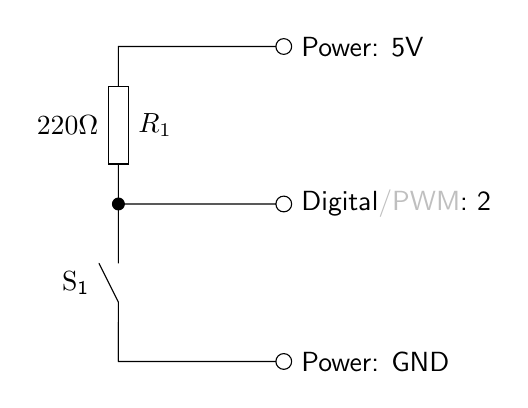
\begin{tikzpicture}[circuit ee IEC]
        % \draw[help lines,step=0.25] grid(10,10);

        % \draw[draw=none,fill=white] (0.5,0.5) rectangle ++(6.5,5);

        \node[anchor=west,font=\sffamily] at (4.2,5) {Power: 5V};
        \node[anchor=west,font=\sffamily] at (4.2,3) {Digital\textcolor{gray!50}{/PWM}: 2};
        \node[anchor=west,font=\sffamily] at (4.2,1) {Power: GND};

        \draw (4.1,5) circle(1mm) ++(-0.1,0) -- ++(-2,0) -- ++(0,-0.5) ++(0,-1) -- ++(0,-0.5) ++(0,-1.5) -- ++(0,-0.5) -- ++(2,0) ++(0.1,0) circle(1mm);
        \draw[fill=black] (2,3) circle(0.75mm);
        \draw (2,3) -- ++(2,0) ++(0.1,0) circle(1mm);
        % \draw (2,3) -- ++(0,-0.5) ++(0,-0.05) circle(0.5mm) ++(0,-0.9) circle(0.5mm);
        % \draw[line width=0.2mm] (2,1.5) ++(-0.03,0.08) -- +(120:0.8);
        % \draw[dashed] (2,1.5) ++(-0.03,0.04) ++(120:0.4) -- ++(-0.5,0);
        % \draw (2,1.5) ++(-0.03,0.04) ++(120:0.4) ++(-0.5,0) ++(0,0.1) -- ++(0,-0.2);
        \node at (2,4) [fill=black!20!yellow!60,resistor,ohm=220,rotate=90,fill=none,info'=$R_{1}$] {};
        \draw (2,1) to [make contact={info={S$\mathsf{_{1}}$}}] (2,3);

          
    \end{tikzpicture}
\end{document}         